\chapter{Resultados y discusión}

\section{Estabilidad de estructuras}

Antes de estudiar la acidez de los compuestos a proponer, se hace un análisis de la estabilidad de sus isómeros y confórmeros con el fin de buscar las estructuras más estables. 
Se estudiarán los posibles isómeros y confórmeros de los ácidos sulfúrico, carbónico y fosfórico (ANEXO X) con el fin de hallar la estructura más estable en fase gas. \\

  \begin{table}[H]
\begin{center}
\begin{tabular}{|c|c|c|c|c|c|}
\hline
Isómeros $H_2SO_4$ & $\Delta E$ & Isómeros $H_2CO_3$ & $\Delta E$ & Isómeros $H_3PO_4$ & $\Delta E$ \\ \hline
$Conf_1$ & 4,1908 & $Conf_1$ & 0,0000 & $Conf_1$ & 0,9832 \\ \hline
$Conf_2$ & 2,5058 & $Conf_2$ & 1,3775 & $Conf_2$ & 0,4458 \\ \hline
$Conf_3$ & 0,0000 & -- & -- & $Conf_3$ & 0,0000 \\ \hline
-- & -- & -- & -- & $Conf_4$ & 0,6187 \\ \hline
\end{tabular}
\caption{Diferencias de la energía libre de Gibbs en Kcal/mol de cada isómero conformacional de los ácidos.}
\label{tab:3.1}
\end{center}
\end{table}
A la vista de los resultados de energías expuestos en la Tabla 3.1, el isómero más estable del ácido sulfúrico es el confórmero 3, debido a que dicha disposición espacial minimiza las repulsiones de los pares de electrones originando una baja energía y a su vez una mayor estabilidad, ésta también se debe a la posible formación de puentes de hidrógeno intramoleculares, ya que los hidrógenos 3 y 7 de dicho confórmero están dirigidos hacia los átomos de oxígeno 5 y 4 respectivamente, con dos pares de electrones libres en orbitales p, la distancia de los H a los O es menor que la suma de sus radios de Van Der Waals, los H presentan una carga positiva y los oxígenos una negativa como se muestra en la figura 3.1. \\
\begin{center} Radios de Van Der Waals en $\Armstrong $
$$O\longrightarrow1,5$$
$$H\longrightarrow1,2
$$
\end{center}
\begin{figure}[H]
	\centering
	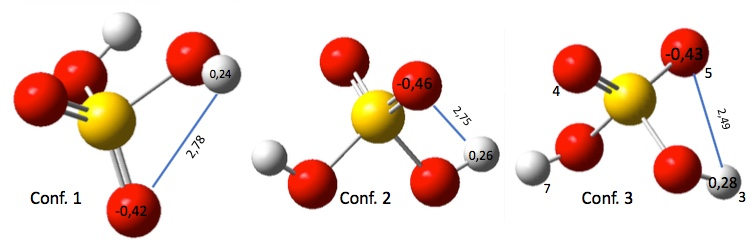
\includegraphics[scale=0.4]{prezimagen}
	\caption{Parámetros para un enlace de hidrógeno, distancias en $\Armstrong$}
\end{figure}

El confórmero del ácido carbónico más estable es el confórmero 1, pero hay que tener en cuenta que la diferencia de energía es mínima, los dos confórmeros presentan una estructura trigonal plana, y un enlace muy fuerte CO, pero dicho confórmero posee una de las otras dos distancias CO menor que en el confórmero 2, Tabla 3.3, por tanto sus enlaces son más fuertes y la molécula presenta menor energía total y mayor estabilidad, tabla \ref{tab:3.1}. 
\begin{table}[H]
    \centering
    \begin{tabular}{|c|c|c|}
    \hline
    Confórmeros del $H_2CO_3$ & $d(C-OH_{(1)})$ & $d(C-OH_{(2)})$ \\ \hline
    $Conf_1$ & 1,34 & 1,34  \\ \hline
    $Conf_2$ & 1,36 & 1,34 \\ \hline 
    \end{tabular}
    \caption{Distancias C-OH del ácido carbónico}
\end{table}

En cuanto a los confórmeros del ácido fosfórico, no se puede decir que el confórmero 3 sea el más estable ya que las diferencias de energía son demasiado pequeñas, y entra dentro del error que puede tener el método teórico usado. Ver tabla \ref{tab:3.1}. Esto es debido a que las cuatro distancias P-O de los confórmeros son relativamente altas y no hay posibilidad de formación de enlaces de hidrógeno para ninguna de las estructuras propuestas.

Se estudia también la estabilidad de los isómeros y confórmeros de los ácidos anteriores sustituyendo uno o varios átomos de hidrógeno por halógenos. Tablas de la 3.3 a la 3.6. Al sustituir un átomo de hidrógeno por un halógeno la distribución de carga de la molécula se verá afectada, y por tanto, la disposición espacial de los átomos, el halógeno podrá asociarse tanto al átomo central como a uno de los oxígenos. Una de las ideas propuestas derivadas de este estudio de  estabilidad, es localizar la estructura más favorable para conseguir evaluar el efecto de la sustitución sobre la acidez. Ver estructuras de todos los isómeros en el ANEXO X.

En primer lugar se estudian los isómeros y confórmeros del ácido sulfúrico sustituido, donde el isómero 2 del $HClSO_4$ tiene dos enlace S-O muy fuerte (d(S-O)=1,43$\Armstrong$) y la disposición del cloro es tal que no hay impedimento estérico ya que está en trans con el hidrógeno. (Ver Fig:3.2). El isómero 8 del $HFSO_4$ es la molécula más estable en la sustitución de un hidrógeno por un átomo de flúor, ya que es la única con dos enlaces S-O muy fuertes (d(S-O)=1,43 $\Armstrong$), además sienten mucha atracción ya que el azufre tiene gran carga natural positiva y los dos oxígenos gran carga negativa (S=2,39 y cada uno de los oxígenos de dicho enlace fuerte -0,81)

\begin{table}[H]
	\begin{center}
		\begin{tabular}{|c|c|c|c|}
			\hline
			Isómeros $HFSO_4$ & $\Delta E$ & Isómeros $HClSO_4$ & $\Delta E$ \\ \hline
			$iso_1$	& 10,818 & $iso_1$ & 0,0555 \\ \hline
			$iso_2$ & 10,777 & $iso_2$ & 0,0000 \\ \hline
			$iso_3$ & 10,780 & $iso_3$ & 65,028 \\ \hline
			$iso_4$ & 10,826 & $iso_4$ & 64,227 \\ \hline
			$iso_5$ & 42,675 & $iso_5$ & 24,428 \\ \hline
			$iso_6$ & 10,826 & $iso_6$ & 0,0427 \\ \hline
			$iso_7$ &	101,31 & $iso_7$ & 109,95 \\ \hline
			$iso_8$ &	0,0000 & $iso_8$ & 4,8299 \\ \hline
		\end{tabular}
		\caption{Diferencias de la energía libre de Gibbs en Kcal/mol de cada isómero conformacional del ácido sulfurico sustituyendo un H por un halógeno}
	\end{center}
\end{table}

Los isómeros más estables del ácido carbónico sustituido con halógenos presentan distancias menores de enlaces C-O, dos isómeros de cada compuesto halogenado presentan hibridación $sp^2$, es decir, enlaces más fuertes, por lo que poseen una energía total menor, por ello la diferencia entre los isómeros 4 y 5 es tan pequeña, en el caso del compuesto de flúor la diferencia es de de 2 Kcal/mol esto puede ser porque el enlace de hidrógeno que se forma es más débil en el isómero 4, ya que el oxígeno que interviene tiene muy cerca el flúor, y por consiguiente una carga menos negativa. Véase la figura 3.2.

\begin{figure}[H]
	\centering
	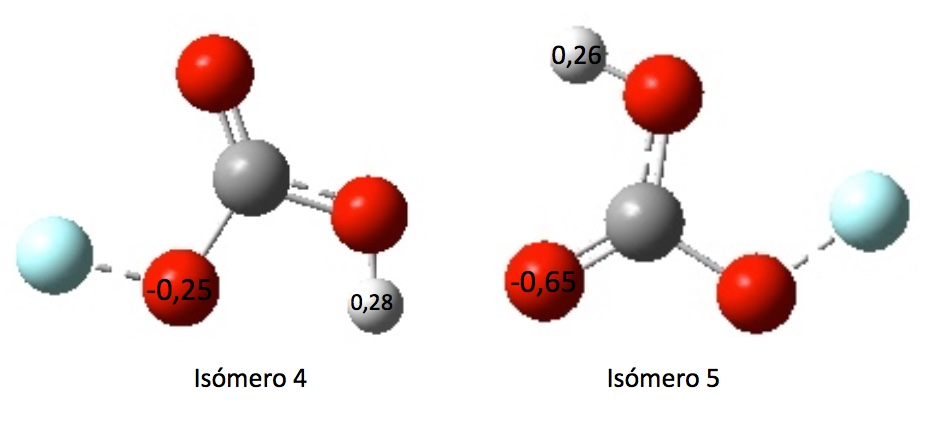
\includegraphics[scale=0.2]{prezimagen3}
	\caption{Isómeros $HFCO_3$}
\end{figure} 

\begin{table}[H]
	\begin{center}
		\begin{tabular}{|c|c|c|c|}
			\hline 
			Isómeros $HFCO_3$ & $\Delta E$ & Isómeros $HClCO_3$& $\Delta E$ \\ \hline
			$Iso_1$ & 3,9632 & $Iso_1$ & 49,890 \\ \hline
			$Iso_2$ & 3,8449 & $Iso_2$ & 48,952 \\ \hline
			$Iso_3$ & 92,693 & $Iso_3$ & 91,991 \\ \hline
			$Iso_4$ & 1,8115 & $Iso_4$ & 0,0000 \\ \hline
			$Iso_5$ & 0,0000 & $Iso_5$ & 0,3151 \\ \hline
		\end{tabular}
		\caption{Diferencias de la energía libre de Gibbs en Kcal/mol de cada isómero conformacional del ácido carbónico sustituyendo un H por un halógeno}
	\end{center}
\end{table}

Análogamente a los casos de los ácidos anteriores se concluye que los compuestos más estables al sustituir un hidrógeno por un halógeno en el ácido fosfórico son el isómero 9 en el caso del $H_2FPO_4$ y en el de $H_2ClPO_4$ el Isómero 3, la estabilidad de éstos se debe a su geometría tretraédrica, los isómeros restantes con dicha estructura son los que no presentan gran diferencia energética (isómeros 1, 2 y 3 para el compuesto con flúor e isómeros 1, 2, 11 y 12 para el de cloro), no es posible explicar la estabilidad del isómero comparada con éstos ya que tenemos que tener en cuenta el error del método. 

\begin{table}[H]
\begin{center}
\begin{tabular}{|c|c|c|c|}
\hline
Isómeros $H_2FPO_4$ & $\Delta E$ & Isómeros $H_2ClPO_4$ & $\Delta E$ \\ \hline
$Iso_1$& 1,2641 & $Iso_1$ & 0,8643 \\ \hline
$Iso_2$ & 1,2640 & $Iso_2$ & 0,8675 \\ \hline
$Iso_3$ & 0,0014 & $Iso_3$ & 0,0000 \\ \hline
$Iso_4$	& 8,6205 & $Iso_4$ & 40,005 \\ \hline
$Iso_5$	& 8,6218 & $Iso_5$ & 40,001 \\ \hline
$Iso_6$	& 56,668 & $Iso_6$ & 29,134 \\ \hline
$Iso_7$	& 8,4010 & $Iso_7$ & 40,725 \\ \hline
$Iso_8$	& 8,6178 & $Iso_8$ & 43,487 \\ \hline
$Iso_9$	& 0,0000 & $Iso_9$ & 29,959 \\ \hline
$Iso_{10}$	& 57,869 & $Iso_{10}$ & 90,161 \\ \hline
$Iso_{11}$ & 22,242 & $Iso_{11}$ & 1,2929 \\ \hline
$Iso_{12}$ & 23,164 & $Iso_{12}$ & 0,5166 \\ \hline
\end{tabular}
\caption{Diferencias de la energía libre de Gibbs en Kcal/mol de cada isómero conformacional del ácido fosfórico sustituyendo un hidrógeno por un halógeno.}
\end{center}
\end{table}

Al sustituir un hidrógeno más por otro halógeno las moléculas de mayor estabilidad son el isómero 1 para el  $HF_2PO_4$, ésto es debido a que es el único isómero que forma un enlace de hidrógeno con el flúor (d(H--F)=2,2$\Armstrong$), en el caso del  $HCl_2PO_4$ el isómero 6, hay que tener en cuenta que hay dos isómeros más de esta última molécula muy parecidos en energía, son las únicas con geometría tetraédrica, en el caso del isómero 6, uno de los cloros esta más alejado del centro {\bfseries(de masas)?} de la molécula, reduciendo el impedimento estérico y aumentando su estabilidad.

\begin{table}[H]
	\centering
	\begin{tabular}{|c|c|c|c|}
		\hline
		Isómeros $HF_2PO_4$ & $\Delta E$   & Isómeros $HCl_2PO_4$ & $\Delta E$     \\ \hline
		$Iso_1$  & 0,000     & $Iso_1$     & 98,649 \\ \hline
		$Iso_2$  & 18,038    & $Iso_2$   & 38,457 \\ \hline
		$Iso_3$   & -- & $Iso_3$    & 39,297 \\ \hline
		$Iso_4$   & --& $Iso_4$    & 39,330 \\ \hline
		$Iso_5$   & -- & $Iso_5$  & 38,462 \\ \hline
		$Iso_6$    & 60,559    & $Iso_6$  & 0,000  \\ \hline
		$Iso_7$   & 60,559    & $Iso_7$   & 2,077  \\ \hline
		$Iso_8$    & 15,887    & $Iso_8$  & 19,523 \\ \hline
		$Iso_9$   & 36,514    & $Iso_9$   & 0,101  \\ \hline
		$Iso_{10}$  & 39,126    & $Iso_{10}$   & 38,645 \\ \hline
	\end{tabular}
\caption{Diferencias de la energía libre de Gibbs en Kcal/mol de cada isómero conformacional del ácido fosfórico sustituyendo dos hidrógenos por dos halógenos.}
\end{table}

Si se observa la tabla 3.6, el vacío de los isómeros 3, 4 y 5 del $HF_2PO_4$ se debe a que las geometrías propuestas no se optimizaron ya que no se llegó a un mínimo de energía.


También se ha realizado el estudio de estabilidad entre dichos ácidos observando el isómero más estable de cada uno, ver tabla 3.7, se tiene que el ácido más estable es el sulfúrico, seguido del fosfórico y por último, el menos estable de los tres, el ácido carbónico \\

\begin{table}[H]
	\centering
	\begin{tabular}{|c|c|c|c|c|c|}
		\hline
Ácido&$\Delta E$&Ácido&$\Delta E$& Ácido&$\Delta E$\\ \hline
$H_2SO_4$&0,00&$HFSO_4$&0&$HClSO_4$&0\\ \hline
$H_3PO_4$&3,52E+04&$H_2FPO_4$&3,52E+04&$H_2ClPO_4$&3,52E+04\\ \hline
$H_2CO_3$&2,73E+05&$HFCO_3$&2,73E+05&$HClCO_3$&2,73E+05\\ \hline
	\end{tabular}
	\caption{Diferencias de energía en Kcal/mol}
\end{table}
Dicha estabilidad se debe a que la estructura del ácido carbónico es plana (trigonal plana) y por lo tanto más rígida, lo que le proporciona menor estabilidad.\\ Sin embargo, las otras dos estructuras son tetraédricas, en el caso del ácido fosfórico, las distancias P-O son mayores que las distancias S-O, ya que el fósforo es de mayor tamaño que el azufre y menos electronegativo, por consiguiente, distancias O--H mayores, sin posibilidad de formar enlaces de hidrógeno en dicha molécula, mientras que en el ácido sulfúrico si se forma dicho enlace. Ver figura 3.3
\begin{figure}[H]
	\centering
	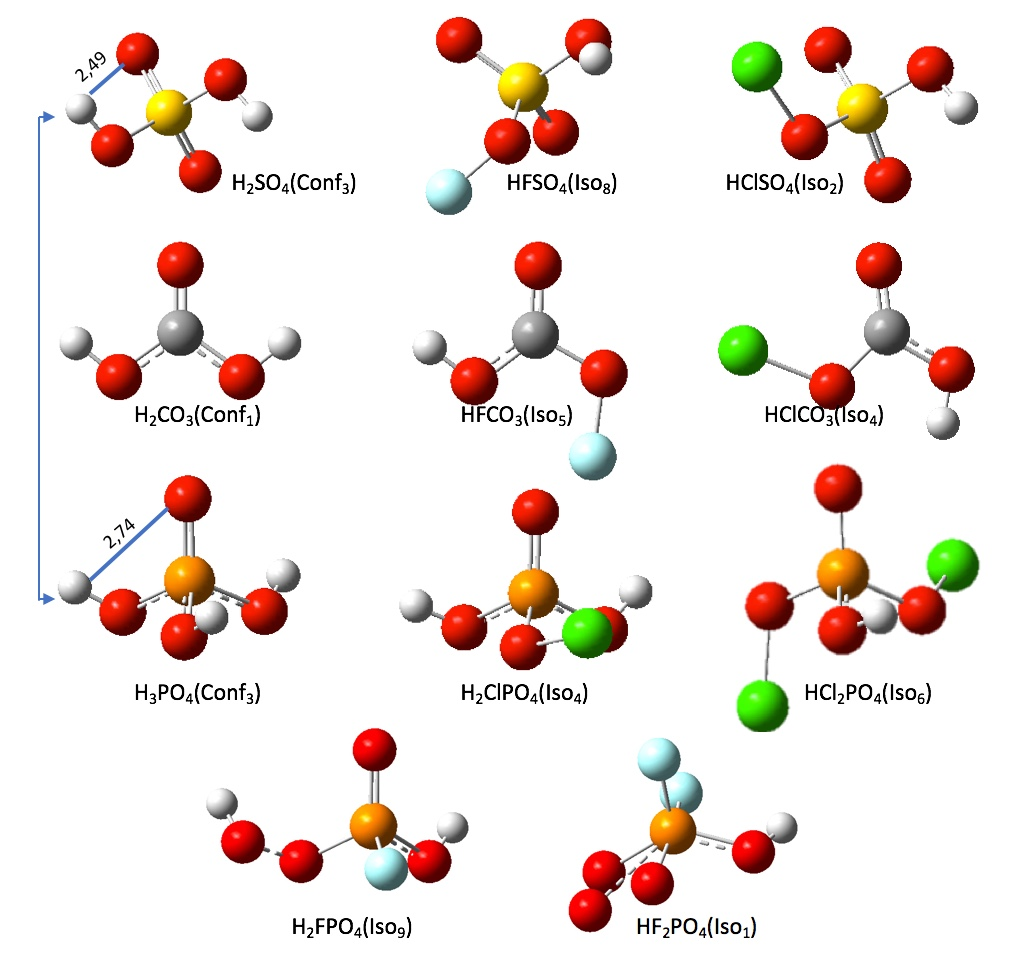
\includegraphics[scale=0.3]{prezimagen2}
	\caption{Isómeros más estables  de los ácidos objeto de estudio.}
\end{figure}

\section{Acidez en fase gas de moléculas}


La acidez en fase gaseosa de un ácido neutro HA se refiere al siguiente equilibrio:

$$HA\xrightleftharpoons{\Delta G} H^+ + A^-$$

Donde $\Delta G$ es la acidez en fase gaseosa, dicha cantidad es de interés fundamental y proporciona informacion valiosa sobre las propiedades intrínsecas, independientes del disolvente de los ácidos. \cite{quimica3}

Con el fin de estudiar el impacto de las sustituciones de hidrógenos por halógenos en la acidez en fase gas de los ácidos, se han diseñado más estructuras sustituyendo hidrógenos por flúor. Para calcular la acidez en fase gas se han hecho los mismos cálculos computacionales con sus aniones. También se ha sustituido el grupo ácido por otro para así ver la variación de acidez.


 \begin{table}[H]
     \centering
     \begin{tabular}{|c|c|c|c|}
     \hline
     \multicolumn{4}{|c|}{\bfseries{ACIDEZ}} \\ \hline
     Ácido & $\Delta G$ & $\Delta G_{exp}$ & $\Delta G_{ H. especf}$ \\ \hline
$CF_3COOH$ & 314,04 & 316,3 & 309,0282809\\ \hline
$CF_3COSH$ & 311,58 & 312,5 & 303,3527667\\ \hline
$CF_3SO_3H$ & 292,87 & 299,5 &292,2881339\\ \hline
$FHSO_3$ & 293,57 & 299,8 & 293,0524411\\ \hline
$H_2CFCOOH$ & 328,14 &-- & 320,5998791\\ \hline
$H_2CFCOSH$ & 323,99 & --& 314,4709262\\ \hline
$H_2CFSO_3H$ & 303,60 & -- & 302,9127567\\ \hline
$H_2CO_3$ & 327,95	& -- & 319,6992767\\ \hline
$H_2S_2O_6$ & 281,75 & -- & 283,4104362\\ \hline
$H_2SO_4$ & 302,60	& 302,2 & 301,2892628\\ \hline
$H_3CCOOH$ & 338,57 & -- &	328,9212264\\ \hline
$H_3CCOSH$ & 330,46 & -- &	319,4866136\\ \hline
$H_3CSO_3H$ & 312,65 & 315,0 & 309,7167849\\ \hline
$HCF_2COOH$ & 	321,43 & -- & 314,9858609\\ \hline
$HCF_2COSH$ & 	316,83 & -- & 308,5712026\\ \hline
$HCF_2SO_3H$ & 	297,86 & -- & 298,3781185\\ \hline
$HPO_3$ & 303,54 & 303,3 & 300,9305154\\ \hline
$HNO_3$ & 315,01 & 317,8 & 309,4734993\\ \hline
$H_3PO_4$ & 321,44	& -- & 332,5547603 \\ \hline
$HF_2PO_4$ & 385,70 & -- &  \\ \hline
$HFSO_4$ & 282,97 & -- &\\ \hline
$HClSO_4$ & 293,26 & -- & 288,50\\ \hline
$HFCO_3$ & 309,08 & -- &\\ \hline
$HClCO_3$ & 312,51 & -- &\\ \hline
$H_2ClPO_4$ & 336,99 & -- &\\ \hline
$HCl_2PO_4$ & 332,23 & -- &\\ \hline
$H_2FPO_4$ & 329,26 & -- &\\ \hline
     \end{tabular}
     \caption{Acideces en fase gas con y sin hidratación específica y el valor experimental en Kcal/mol. $\cite{quimica3}$ }
     \label{tab:3.9}
 \end{table}

Se han estudiado distintos tipos de ácidos, por un lado, los oxácidos estudiados en la parte 1 del presente trabajo añadiendo alguno más y, por otro lado, algunos ácidos orgánicos de interés, así se hace un estudio de acidez en fase gaseosa más extenso y riguroso.
 
 Los resultados dados en la Tabla 3.8 apoyan el siguiente orden de acidez intrínseca para los ácidos orgánicos: $ CF_3SO_3H>HCF_2SO_3H>H_2CFSO_3H>CF_3COSH>H_3CSO_3H>CF_3COOH>HCF_2COSH>HCF_2COOH>H_2CFCOSH>H_2CFCOOH>H_3CCOSH>H_3COOH $, y el siguiente para los oxácidos: $ H_2S_2O_6>FHSO_3>H_2SO_4>HPO_3>HNO_3>H_3PO_4>H_2CO_3 $.

Los ácidos llamados normalmente fuertes ($ CF_3SO_3H$, $FHSO_3$, $HCF_2SO_3H$, $H_2SO_4$, $HPO_3$, $H_2CFSO_3H$) están en un intervalo de acidez relativamente estrecho (10,7 kcal/mol), se tienen algunos valores experimentales, donde la variación con los calculados computacionalmente no llega a las 3 Kcal/mol exceptuando al $CF_3SO_3H$ y al $FHSO_3$ que difieren de 6-7 kcal/mol, al tener una diferencia tan alta, se ha llevado a cabo un cálculo G4 para estos dos últimos ácidos con el fin de ver si el primer cálculo sobreestima la acidez de dichos ácidos. 
\begin{table}[H]
	\centering
	\begin{tabular}{|c|c|c|}
		\hline
		Ácido & $\Delta G$ & $\Delta G_{exp}$ \\ \hline
		$CF_3SO_3H$ &{\bfseries dato }& 299,5 \\ \hline
		$FHSO_3$ & 294,8 & 299,8 \\ \hline 
	\end{tabular}
\caption{Acideces en fase gas con el método G4 en Kcal/mol}
\end{table}

En vista de los resultados obtenidos con el método compuesto G4 se observa como la acidez no varía prácticamente nada (1,5Kcal/mol) en comparación con el cálculo DFT, pero podemos decir que dicho método sobreestima la acidez de dichos compuestos y como era de esperar, el método G4 describe mejor su acidez que el método DFT B3LYP/6-311G**.

La acidez es proporcional a la tendencia del ácido a perder un protón. Se ve como el orden de acidez sustituyendo el grupo ácido es $ COOH {<} COSH {<} SO3H $, ya que en los aniones correspondientes se debe tener en cuenta la estabilización por resonancia, deslocalización de enlaces $\pi$, que es mayor en el $SO3^-$ ya que hay mayor número de átomos, en cuanto a las otras dos estructuras, los iones $COS^-$ y $COO^-$ son estabilizados por resonancia, pero en el $COS^-$ es mayor, se puede explicar observando la carga natural en dichos átomos dada en la tabla 3.10. Ver figura 3.4.

\begin{figure}[H]
	\centering
	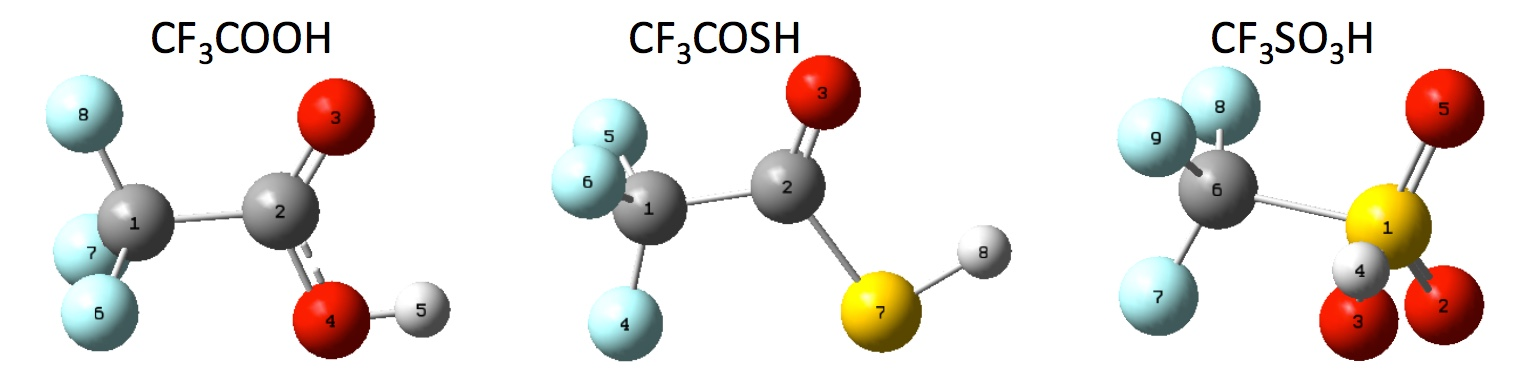
\includegraphics[scale=0.2]{CF3-grupo}
	\caption{Ácidos con tres átomos de flúor}
\end{figure}

\begin{table}[H]
    \centering
    \begin{tabular}{|c|c|c|c|c|c|}
    \hline
    $SO3^-$ & Carga Natural &$COS^-$ & Carga Natural & $COO^-$ & Carga Natural \\ \hline
    S & 2.21439 & C & 0.22678 & C & 0.68743 \\ \hline
    O & -0.97579 & O & -0.61533 & O & -0.73587 \\ \hline
    O & -0.97575 & S & -0.48786 & O & -0.74097 \\ \hline
    O & -0.97579 & -- & -- & -- & -- \\ \hline
    \end{tabular}
    \caption{Cargas naturales de la moléculas $CF_3-$ grupo ácido}
\end{table}

Comparamos también sustitución de átomos de flúor por átomos de hidrógeno en el grupo $CF_3$ de la molécula. En la tabla \ref{tab:3.9} se ve que cuantos más átomos de flúor haya en la molécula mayor es su acidez, esto se debe a la elevada electronegatividad del flúor, cuántos más átomos de flúor haya, mayor capacidad atractora tendrá el grupo, y mayor será el efecto inductivo, polarización de carga transmitida por enlaces $\sigma$, si se observa la distancia O-H de cada molécula (tabla 3.12) se comprueba la facilidad de romper dicho enlace en presencia de átomos electronegativos.

\begin{figure}[H]
	\centering
	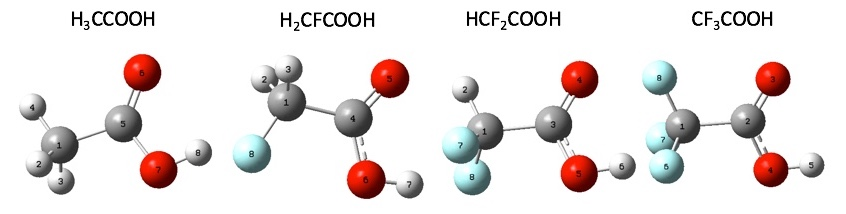
\includegraphics[scale=0.4]{grupo-COOH}
	\caption{Ácidos carboxílicos con diferentes sustituciones de hidrógenos por átomos de flúor.}
\end{figure}
\begin{table}
	\centering
	\begin{tabular}{|c|c|}
		\hline
		Ácido & d(O-H)
		
	\end{tabular}
\end{table}
\begin{table}[H]
    \centering
    \begin{tabular}{|c|c|c|c|c|c|c|c|}
    \hline
    $CF_3-$ & Carga Mull & $HCF_2-$ & Carga Mull & $H_2CF-$ & Carga Mull & $H_3C-$ & Carga Mull \\ \hline
     C & 0.549474 &  C & 0.382878 & C & 0.151906 & C & -0.189412 \\ \hline
     C & 0.201081 &  C & 0.204525 & C & 0.203532 & C & 0.234883 \\ \hline
     O & -0.482870 & O & -0.510709 & O & -0.527054 & O & -0.519973 \\ \hline
     O & -0.491545 & O & -0.488498 &  O & -0.493739 & O & -0.525498 \\ \hline
     F & -0.261497 & F & -0.287967 & F & -0.334645 &  & \\ \hline
     F & -0.261531 & F & -0.300230 &  &  &  & \\ \hline
     F & -0.253112 &  &  &  &  &  & \\ \hline
    \end{tabular}
    \caption{Carga Mulliken de moléculas grupo-COOH con las cargas de hidrógenos sumadas dentro de los átomos pesados.}
\end{table}

\subsection{Hidratación específica}
Se estudia el impacto que tiene la hidratación específica en la acidez de las moléculas anteriores, en la tabla \ref{tab:3.9} también se indica la acidez en presencia de una molécula de agua en fase gas.
A la vista de los resultados expuestos, la acidez aumenta al haber una molécula de agua en un punto determinado de la molécula, ya que se forman enlaces de hidrógeno fuertes como se puede comprobar mirando las distancias d(O-H) y teniendo en cuenta la existencia de un máximo de densidad en dichos enlaces en la tabla 3.13. 

{\bfseries TENGO QUE MIRAR DETENIDAMENTE EL H3PO4 Y H3PO4-H2O}

\begin{table}[H]
	\centering
	\begin{tabular}{|c|c|c|c|}
		\hline
		Ácidos-$H_2O$ & distancia	& d(O-H) ($\Armstrong$) & $Max_{densidad}$ \\ \hline
		$CF_3COOH-H_2O$ & $d(O_9-H_5)$ &1,6926&4,665E-02\\ \cline{2-4}
& $d(O_3-H_{10})$ & 2,1371 & 1,852E-02 \\ \hline
 $CF_3COSH-H_2O$ & $d(O_9-H_8)$	 & 1,9225 & 3,014E-02 \\ \cline{2-4}
	& $d(O_3-H_{10})$ & 2,0486 & 2,064E-02 \\ \hline
	$CF_3SO_3H-H_2O$ & $d(O_{10}-H_4)$ & 1,6142 & 5,653E-02 \\ \cline{2-4}
	& $d(O_5-H_{12})$	& 2,1910 &	1,631E-02 \\ \hline
 $FHSO_3-H_2O$	& $d(O_7-H_4)$ & 1,6098 &	5,682E-02 \\ \cline{2-4}
	& $d(O_5-H_8)$	& 2,3134	& 1,323E-02 \\ \hline
 $H_2CFCOOH-H_2O$	&$d(O_9-H_7)$ & 1,7347	& 4,251E-02 \\ \cline{2-4}
	& $d(O_5-H_{11})$ & 2,0119	& 2,375E-02 \\ \hline
 $H_2CFCOSH-H_2O$ &	$d(O_3-H_{10})$ & 1,9847 &	2,356E-02 \\ \cline{2-4}
	& $d(O_9-H_6)$ & 1,9897	& 2,633E-02 \\ \hline
 $H_2CFSO_3H-H_2O$ &	$d(O_{10}-H_4)$	& 1,6489	& 5,205E-02 \\ \cline{2-4}
	& $d(O_5-H_{11})$ & 2,0786	& 2,015E-02 \\ \hline
 $H_2CO_3-H_2O$	& $d(O_7-H_5)$	& 1,7367	& 4,163E-02 \\ \cline{2-4}
	& $d(O_2-H_9)$ & 2,2011	& 1,575E-02 \\ \hline
 $H_2S_2O_6-H_2O$ &	$d(O_{11}-H_{10})$	& 1,5480 &	6,753E-02 \\ \cline{2-4}
	& $d(O_2-H_{12})$ & 2,0478 &	1,959E-02 \\ \hline
 $H_2SO_4-H_2O$	& $d(O_8-H_5)$ & 1,6514	& 5,181E-02 \\ \cline{2-4}
	& $d(O_6-H_9)$ & 2,1459	& 1,768E-02 \\ \hline
 $H_3CCOOH-H_2O$ & $d(O_9-H_8)$ & 1,7673	& 3,947E-02 \\ \cline{2-4}
	& $d(O_6-H_{10})$ & 1,9607 &	2,645E-02 \\ \hline
 $H_3CCOSH-H_2O$ &	$d(O_3-H_{10})$	& 1,9582 &	2,496E-02 \\ \cline{2-4}
	& $d(O_9-H_5)$	& 1,9999	& 2,587E-02 \\ \hline
 $H_3CSO_3H-H_2O$	& $d(O_{10}-H_4)$	& 1,6892	& 4,736E-02 \\ \cline{2-4}
	& $d(O_5-H_{11})$	& 2,0648 &	2,080E-02 \\ \hline
 $HCF_2COOH-H_2O$	& $d(O_9-H_6)$	&1,7146	& 4,446E-02 \\ \cline{2-4}
	& $d(O_4-H_{11})$ & 2,0782	& 2,083E-02 \\ \hline
 $HCF_2COSH-H_2O$	& $d(O_9-H_7)$ &1,9489 & 2,858E-02 \\ \cline{2-4}
	& $d(O_3-H_{10})$ & 2,0214 &	2,186E-02 \\ \hline
 $HCF_2SO_3H-H_2O$	& $d(O_{10}-H_4)$ & 1,6342	& 5,386E-02 \\ \cline{2-4}
&	$d(O_5-H_{12})$ & 2,1099	& 1,899E-02 \\ \hline
 $HPO_3-H_2O$	& $d(O_6-H_2)$ & 1,6586	& 5,063E-02 \\ \cline{2-4}
	& $d(O_4-H_7)$ & 2,1034	& 1,920E-02 \\ \hline
 $HNO_3-H_2O$	& $d(O_6-H_2)$	& 1,6767	& 4,803E-02 \\ \cline{2-4}
	& $d(O_4-H_7)$ & 2,2611	& 1,515E-02 \\ \hline
	\end{tabular}
\caption{Análisis de enlaces de hidrógeno en los ácidos objeto de estudio}
\end{table}
\begin{figure}[H]
	\centering
	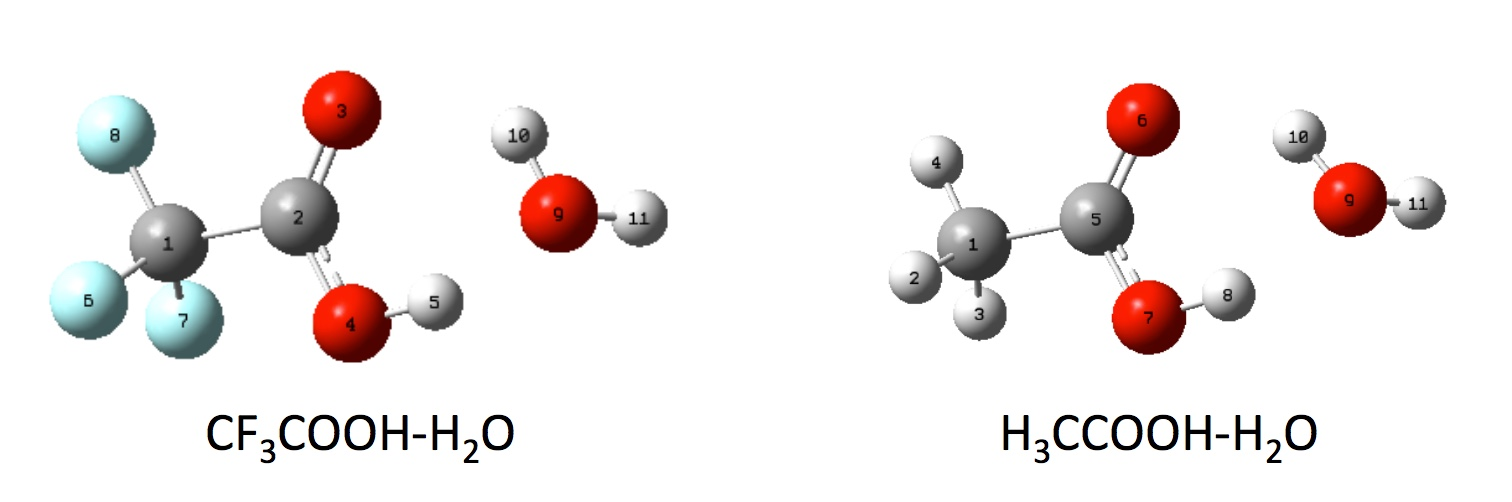
\includegraphics[scale=0.2]{acidos-h2o}
	\caption{Ácidos-$H_2O$}
\end{figure}
 Teniendo en cuenta el análisis NBO de dichas moléculas también comprobamos la mayor facilidad para romper el enlace O-H cuando se expone el ácido a la hidratación específica. En la molécula $H_3COOH$, los dos pares libres de electrones del átomo $O_7$ donan 5,69 y 44,35 Kcal/mol al enlace $C_5=O_6$ mientras que en la molécula de $H_3COOH-H_2O$, al formar un enlace de hidrógeno, los pares libres del $O_7$ donan 7,28 y 53,66 Kcal/mol, por lo que el enlace O-H se debilita, y en consecuencia aumenta la acidez de dicha molécula.
 La diferencia de acidez entre el $CF_3COOH$ y el $H_3COOH$ es de 24,53 Kcal/mol, hidratando los ácidos de forma específica ($CF_3COOH-H_2$ y $H_3COOH-H_2O$) la diferencia se reduce a 19,89 Kcal/mol. Esto lleva a pensar que el efecto del agua en ese punto, en el ácido trifluoretanoico, no es completo, puesto que el efecto inductivo del los tres halógenos compite con este. En el caso del ácido etanoico, al no tener efecto inductivo por parte de ninugn halógeno, el incremento de la acidez de dicho ácido es mayor al ser hidratado.
 Se ven algunas de las distancias de dichos ácidos en la tabla 3.14.
 \begin{table}[H]
 	\centering
 	\begin{tabular}{|c|c|c|c|c|c|c|}
 		\hline
 			 & d(C-F)	& d(O-H) & d(C=O) & & d(O-H) & d(C=O) \\ \hline
$CF_3COOH$ & 1,34 & 0,97 & 1,19 & $H_3CCOOH$ & 0,97 &1,21 \\ \hline $CF_3COOH-H_2O$	& 1,34 & 0,99 & 1,21 & $H_3CCOOH-H_2O$	& 0,99 &1,22 \\ \hline
 	\end{tabular}
 \caption{Distancias internucleares de interés de cada ácido en $\Armstrong$}
 \end{table}
Las d(C-F) son las mismas para las dos moléculas, en las demás distancias se observa una pequeña variación, haciendo uso del análisis NBO se ve que un par de electrones libre del $O_9$ de la molécula de $CF_3COOH-H_2O)$ actúa como donador de 24,26 Kcal/mol al enlace $O_4 - H_5$, actuando este último como aceptor. En contraste, en la molécula $H_3COOH-H_2O$, uno de los pares de electrones libres del $O_9$ dona 18,59 Kcal/mol de energía al enlace $O_7-H_8$. Y la energía donada por uno de los pares de electrones libres de los átomos de oxígeno $O_4 y O_7$ respectivamente, a los enlaces C=O correspondientes, es mayor en el ácido $CF_3COOH-H_2O$ que en el $H_3CCOOH-H_2O$.
